\chapter{Black Holes, Photon Orbits, and the Horizon}

Susskind opens this lecture by saying, in effect, that we have only barely begun the Schwarzschild black hole. So he starts over in the right place: not with Einstein's equations, but with the physical contrast between Newtonian point-mass gravity and its relativistic analog. From there the lecture unfolds in a very deliberate rhythm. We first learn what is genuinely special about \(r=2MG\) and \(r=0\); then we pause the infall story to solve a second problem, the circular motion of particles and photons; and only after that do we return to the horizon itself, where a near-horizon change of coordinates reveals why the horizon can look singular in Schwarzschild coordinates and yet be locally mild. These notes follow Leonard Susskind's lecture closely and are prepared in the Video2Book workflow with curation support from LazyingArt LLC.

\section{Point Masses, Idealizations, and Why Black Holes Matter}

The Schwarzschild solution is introduced as an idealization. In Newtonian gravity the force law
\begin{equation}
F=\frac{GMm}{r^{2}}
\end{equation}
already assumes that the gravitating mass is concentrated at a point. Outside a spherical body that is a good approximation; inside real matter it is not. More importantly, real matter resists compression. One never really reaches an infinitely concentrated point center in ordinary Newtonian physics.

That is the background against which the lecture makes its first sharp claim. In Newtonian mechanics a point center is not merely idealized; it is also hard to hit. A perfectly radial trajectory reaches the center, but any arbitrarily small deviation produces angular momentum, and that angular momentum generates the familiar centrifugal barrier. The particle swings around the center rather than going through it. In that sense it is infinitely unlikely that an infalling point particle actually strikes the Newtonian center.

General relativity changes the story. A black hole is the corresponding relativistic point-mass idealization, but the geometry is stronger than the Newtonian force picture. Near the center it can overwhelm the centrifugal barrier itself. The lecture does not yet derive that fact from the field equations; it begins by insisting that we learn to read it directly from the geometry.

\section{The Schwarzschild Metric as the Target Geometry}

The Schwarzschild metric is therefore taken as a target, not yet as a derived result:
\begin{equation}
d\tau^{2}
=
\left(1-\frac{2MG}{r}\right)dt^{2}
-
\left(1-\frac{2MG}{r}\right)^{-1}dr^{2}
-
r^{2}d\Omega^{2}.
\end{equation}
Later the course will return and ask what equations this metric solves. Here the task is simpler and more immediate: what does this geometry mean?

Far away from the gravitating body, \(2MG/r\) is negligible, so the metric becomes ordinary flat spacetime written in polar coordinates. The interesting structure is concentrated at two radii:
\begin{equation}
r=2MG
\qquad \text{and} \qquad
r=0.
\end{equation}
Susskind wants us to keep those two radii conceptually distinct from the start.

\begin{remark}
In the spoken lecture the angular metric is written schematically in a nonstandard convention and then immediately reduced to motion in a single plane. Since the orbit calculation that follows only uses one surviving angular variable, we will denote that angle by \(\theta\) and write the reduced angular term simply as \(r^{2}d\theta^{2}\).
\end{remark}

If we draw time vertically and space horizontally, then \(r=0\) sits at the center of the picture, just as the center of a Newtonian point-particle picture would. Around it there is a cylindrical shell at \(r=2MG\), the Schwarzschild radius, the horizon. Something appears to happen there -- or perhaps only appears to happen there.

The reason for the hesitation is already visible in the metric. At \(r=2MG\), the coefficient of \(dt^{2}\) goes to zero while the coefficient of \(dr^{2}\) blows up. In these coordinates something looks singular. But the lecture makes an immediate distinction:
\begin{itemize}
\item At \(r=2MG\), the pathology is a pathology of Schwarzschild coordinates.
\item At \(r=0\), the pathology is physical.
\end{itemize}

At the center, curvature becomes infinite. In the lecture this is translated into a more physical language: curvature means tidal force. An object falling to \(r=0\) is stretched radially and squeezed transversely without bound. The singularity at \(r=0\) is not a harmless coordinate accident; it is a genuine catastrophe.

\section{Radial Infall, Coordinate Time, and Proper Time}

Having separated horizon from singularity, the lecture briefly recaps radial infall. The point here is not to do integrals; it is to prepare the reader for the later pictures.

For a static clock with \(dr=d\Omega=0\), the metric gives
\begin{equation}
d\tau
=
\sqrt{1-\frac{2MG}{r}}\,dt.
\end{equation}
Very far from the hole we have
\begin{equation}
d\tau\approx dt.
\end{equation}
So far away, proper time and Schwarzschild coordinate time practically agree. But as we move inward, the same coordinate interval \(dt\) corresponds to a smaller and smaller proper-time interval \(d\tau\).

This is the beginning of the infall paradox. In Schwarzschild coordinate time, an object falling toward the horizon takes an infinite time to get there. Its worldline asymptotes to the horizon. Yet the proper time along that worldline need not be infinite. In fact, the infalling observer reaches the horizon in a finite proper time.

The lecture briefly imagines an extended object -- even a meter stick turned into a light clock by putting mirrors at its ends -- and then strips the issue down to its secure core. Whatever clock one builds, whether it is a mechanical clock, a light clock, a heartbeat, or the brain itself, it measures proper time. Proper time is the ticking of a moving clock. Coordinate time is the external bookkeeping variable used to describe the whole geometry.

So before any new causal diagram appears, the tension is already present. In Schwarzschild time the horizon is never reached. In the infaller's own timekeeping it is reached after a finite duration. The lecture will insist later that these are not competing facts; they are descriptions using different clocks.

\section{Circular Motion from the Action Principle}

At this point Susskind changes gears very explicitly. Before returning to the pictures of infall, he wants to solve another problem: orbiting the black hole. That pivot matters. It lets him bring in the machinery of classical mechanics and show that the earlier material on action principles and conservation laws remains useful.

He begins where he likes to begin: with the action. The mass factor in front is not decoration; it is what gives the action the units of energy times time. Writing
\begin{equation}
\mathcal F(r)=1-\frac{2MG}{r},
\qquad
\mathcal G(r)=\mathcal F(r)^{-1},
\end{equation}
and restricting to motion in a fixed plane with one angular variable \(\theta\), we have
\begin{equation}
d\tau
=
dt\,
\sqrt{\mathcal F(r)-\mathcal G(r)\dot r^{\,2}-r^{2}\dot\theta^{\,2}}.
\end{equation}
Therefore
\begin{equation}
S
=
-m\int d\tau
=
-m\int dt\,
\sqrt{\mathcal F(r)-\mathcal G(r)\dot r^{\,2}-r^{2}\dot\theta^{\,2}},
\end{equation}
and the Lagrangian is
\begin{equation}
\mathcal L
=
-m\sqrt{\mathcal F(r)-\mathcal G(r)\dot r^{\,2}-r^{2}\dot\theta^{\,2}}.
\end{equation}

\begin{figure}[h]
\centering

\includegraphics[width=0.70\textwidth]{lecture_06_figure_02.png}
\caption{Relativistic particle Lagrangian in square-root form. The board shows the Lagrangian line itself, while the full expression under the square root is reconstructed cautiously from the lecture.}
\end{figure}

The screenshot is useful precisely because it captures the board hierarchy: first the symbol \(\mathcal L\), then the factor of \(-m\), then the square-root form. The interior of the root is too cropped to trust visually, so the cleaned formula above is transcript-backed rather than purely image-read.

Now comes the mechanics. The conjugate momentum associated with any coordinate \(q\) is
\begin{equation}
p_{q}=\frac{\partial\mathcal L}{\partial \dot q}.
\end{equation}
Applying that once to \(\theta\) and once to \(r\), we find
\begin{align}
L
&=
\frac{\partial\mathcal L}{\partial \dot\theta}
=
\frac{mr^{2}\dot\theta}
{\sqrt{\mathcal F(r)-\mathcal G(r)\dot r^{\,2}-r^{2}\dot\theta^{\,2}}}, \\
p_{r}
&=
\frac{\partial\mathcal L}{\partial \dot r}
=
\frac{m\mathcal G(r)\dot r}
{\sqrt{\mathcal F(r)-\mathcal G(r)\dot r^{\,2}-r^{2}\dot\theta^{\,2}}}.
\end{align}

The radial momentum is not conserved, because radial forces exist. But \(\theta\) is a cyclic coordinate, so \(L\) is conserved. And because the Lagrangian has no explicit time dependence, the Hamiltonian
\begin{equation}
E=H=\sum_{i}p_{i}\dot q_{i}-\mathcal L
\end{equation}
is also conserved. Carrying out the standard construction gives
\begin{align}
E
&=
p_{r}\dot r+L\dot\theta-\mathcal L \\
&=
\frac{m\mathcal G(r)\dot r^{\,2}}{\sqrt{\Delta}}
+
\frac{mr^{2}\dot\theta^{\,2}}{\sqrt{\Delta}}
+
m\sqrt{\Delta} \\
&=
\frac{m\mathcal F(r)}
{\sqrt{\mathcal F(r)-\mathcal G(r)\dot r^{\,2}-r^{2}\dot\theta^{\,2}}},
\end{align}
where
\begin{equation}
\Delta=\mathcal F(r)-\mathcal G(r)\dot r^{\,2}-r^{2}\dot\theta^{\,2}.
\end{equation}

This is exactly the stage in the lecture where Susskind says physics alternates between principles and boring calculations. The point of the principles is that they let us avoid solving more differential equations than we need.

\subsection{Question \& Answer}

\paragraph{Why are angular momentum and energy the right conserved quantities to organize the orbit problem?}

Because the geometry has handed them to us. The coordinate \(\theta\) does not appear explicitly in the Lagrangian, so its conjugate momentum is conserved. The coordinate \(t\) does not appear explicitly either, so the Hamiltonian is conserved. Once those two constants of motion are known, the orbit problem can be reorganized around them. This is why Susskind does not press on with Euler--Lagrange equations here. The conservation laws are the efficient route.

\section{The Photon Sphere from the Effective Energy}

The lecture now specializes to circular motion:
\begin{equation}
\dot r=0.
\end{equation}
Susskind factors the mass out of the angular momentum and introduces the reduced angular momentum
\begin{equation}
\lambda:=\frac{L}{m}.
\end{equation}
The symbol on the board looks somewhat \(\Lambda\)-like, but his spoken notation is clearly ``lambda,'' so we normalize it that way. For a circular orbit the conserved quantities become
\begin{align}
\frac{L}{m}
&=
\frac{r^{2}\dot\theta}
{\sqrt{\mathcal F(r)-r^{2}\dot\theta^{\,2}}}
=
\lambda, \\
E
&=
\frac{\mathcal F(r)m}
{\sqrt{\mathcal F(r)-r^{2}\dot\theta^{\,2}}}.
\end{align}

\begin{figure}[h]
\centering

\includegraphics[width=0.78\textwidth]{lecture_06_figure_04.png}
\caption{Angular momentum and energy for circular Schwarzschild motion. The right board places the reduced angular momentum above the energy, exactly the order needed for the elimination of \(\dot\theta\).}
\end{figure}

The surviving frame is especially useful here because it preserves the lecture's vertical logic. First solve the angular-momentum relation. Then substitute into the energy relation. The left board still carries the generic reminder \(p_{q}=\partial \mathcal L/\partial \dot q\); the right board carries the Schwarzschild-specific content.

Susskind explicitly says he is going to skip the algebraic drudgery and tell us the prescription. We can afford to write the clean version. Squaring the angular-momentum formula gives
\begin{equation}
\lambda^{2}\left(\mathcal F-r^{2}\dot\theta^{\,2}\right)=r^{4}\dot\theta^{\,2},
\end{equation}
so
\begin{equation}
\dot\theta^{\,2}
=
\frac{\lambda^{2}\mathcal F(r)}{r^{2}\left(r^{2}+\lambda^{2}\right)}.
\end{equation}
Substituting this into the energy yields
\begin{align}
E(r,\lambda)
&=
\frac{\mathcal F(r)m}
{\sqrt{\mathcal F(r)-r^{2}\dot\theta^{\,2}}} \\
&=
m\,\frac{\sqrt{\mathcal F(r)}\sqrt{r^{2}+\lambda^{2}}}{r}.
\end{align}

Now comes the specifically relativistic question: can a photon orbit the black hole? Near the Earth, no such effect occurs; the gravitational field is far too weak. To get anything like a circular light orbit one would have to compress the mass down near its Schwarzschild radius. For a black hole, however, the question becomes meaningful.

\begin{figure}[h]
\centering
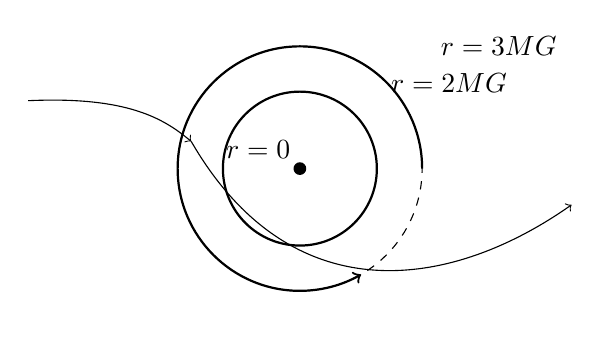
\begin{tikzpicture}[scale=1.15]
\draw[thick] (0,0) circle (0.85);
\draw[dashed] (0,0) circle (1.35);
\fill (0,0) circle (2pt);
\draw[->,thick] (1.35,0) arc (0:300:1.35);
\draw[->] (-3.0,0.75) .. controls (-1.9,0.80) and (-1.5,0.55) .. (-1.20,0.30);
\draw[->] (-1.20,0.30) .. controls (-0.10,-1.60) and (1.65,-1.35) .. (3.0,-0.40);
\node[right] at (0.90,0.95) {\(r=2MG\)};
\node[right] at (1.45,1.35) {\(r=3MG\)};
\node[above left] at (0,0) {\(r=0\)};
\end{tikzpicture}
\caption{Transcript-backed top-down schematic of the horizon, the photon sphere, and a bent light ray. The equation-centered screenshots do not preserve this picture, so the diagram is reconstructed from the lecture narrative.}
\end{figure}

The delicate point is the massless limit. If \(m\to 0\) while \(\lambda\) is held fixed, then the physical angular momentum \(L=m\lambda\) would go to zero, which is not the problem of interest. The correct limit is
\begin{equation}
m\to 0,
\qquad
\lambda\to\infty,
\qquad
L=m\lambda
\quad \text{fixed}.
\end{equation}
In this limit the \(\lambda^{2}\) term dominates inside the square root, and the energy reduces to
\begin{equation}
E_{\gamma}(r;L)
=
L\,\frac{\sqrt{1-\frac{2MG}{r}}}{r}.
\end{equation}
The important point, emphasized in the lecture, is that \(L\) has factored out. The location of the orbit does not depend on the photon's angular momentum.

\subsection{Question \& Answer}

\paragraph{Why does extremizing the energy locate the photon orbit, and why is the extremum a maximum rather than a minimum?}

Once the velocities have been eliminated, we are left with an effective energy for the radial degree of freedom alone. For fixed angular momentum, a circular orbit is an equilibrium condition in \(r\). So we look for a stationary point of
\begin{equation}
\frac{\sqrt{1-\frac{2MG}{r}}}{r}.
\end{equation}
Differentiating gives
\begin{equation}
\frac{d}{dr}
\left(
\frac{\sqrt{1-\frac{2MG}{r}}}{r}
\right)
=
-\frac{\sqrt{1-\frac{2MG}{r}}}{r^{2}}
+
\frac{MG}{r^{3}\sqrt{1-\frac{2MG}{r}}}.
\end{equation}
Setting the derivative to zero yields
\begin{equation}
r=3MG.
\end{equation}

The extremum is a maximum. So the orbit is an equilibrium, but an unstable one. A photon exactly at \(r=3MG\) can circle forever. A photon just outside the top of the effective-energy curve swings around and eventually escapes. A photon just inside it may orbit a few times, but it is pulled inward. This is precisely the lecture's physical picture of the photon sphere.

That same picture immediately explains the optical discussion that follows. A black hole does not simply shift background images outward. Rays can arrive by several different routes; they can wrap around the hole one or many times; they can produce doubles, rings, and an increasingly complicated fragmentation of the background. The full imaging problem is, as Susskind says, a mess, but the circular-orbit calculation already tells us why the mess exists.

The lecture also makes one more qualitative point here. There are no circular photon orbits except this one at \(r=3MG\). More generally, no circular orbit survives inside the photon sphere. Outside it, massive particles can have circular orbits; for massless particles, only the photon sphere remains.

\section{Near the Horizon: Rindler Coordinates and the Exchange of Space and Time}

After the photon sphere, the lecture returns to the original puzzle. The horizon is still peculiar. Clock comparisons blow up there, and the signs of the Schwarzschild coefficients change there. So how can the horizon be both special and locally harmless?

The method is to zoom in. Susskind suppresses the angular directions and chooses units in which
\begin{equation}
2MG=1.
\end{equation}
Then the \(t\)-\(r\) part of the metric becomes
\begin{equation}
d\tau^{2}
=
\left(1-\frac{1}{r}\right)dt^{2}
-
\left(1-\frac{1}{r}\right)^{-1}dr^{2}.
\end{equation}
Now rewrite the Schwarzschild factor as
\begin{equation}
1-\frac{1}{r}=\frac{r-1}{r}.
\end{equation}
Near the horizon \(r=1\), the numerator \(r-1\) must be kept -- it is the small quantity that matters -- but the denominator \(r\) is harmless and can be replaced by its horizon value. Thus, very close to the horizon,
\begin{equation}
d\tau^{2}
\approx
(r-1)\,dt^{2}
-
\frac{dr^{2}}{r-1}.
\end{equation}
Define the distance-from-horizon coordinate
\begin{equation}
\xi=r-1,
\qquad
d\xi=dr.
\end{equation}
Then
\begin{equation}
d\tau^{2}
=
\xi\,dt^{2}
-
\frac{d\xi^{2}}{\xi}.
\end{equation}

This is where the lecture invokes the equivalence principle and goes back to uniformly accelerated coordinates in flat spacetime. In Minkowski coordinates \((X,T)\), define
\begin{equation}
X=\rho\cosh\omega,
\qquad
T=\rho\sinh\omega.
\end{equation}
Then
\begin{equation}
X^{2}-T^{2}=\rho^{2},
\end{equation}
so constant \(\rho\) are hyperbolae. The flat metric becomes
\begin{equation}
d\tau^{2}
=
\rho^{2}d\omega^{2}-d\rho^{2}.
\end{equation}
Now make the purely convenient redefinitions
\begin{equation}
\rho^{2}=4\xi,
\qquad
\omega=\frac{t}{2}.
\end{equation}
Differentiating the first relation gives
\begin{equation}
2\rho\,d\rho=4\,d\xi,
\end{equation}
hence
\begin{equation}
d\rho^{2}=\frac{d\xi^{2}}{\xi}.
\end{equation}
Substituting back, one finds again
\begin{equation}
d\tau^{2}
=
\xi\,dt^{2}
-
\frac{d\xi^{2}}{\xi}.
\end{equation}

So the near-horizon Schwarzschild metric is the Rindler form of flat spacetime. That is the lecture's precise mathematical statement that the horizon is locally mild.

\subsection{Question \& Answer}

\paragraph{How can something happen at the horizon and yet nothing locally dramatic happen there?}

Because the two statements refer to different kinds of structure. In Schwarzschild coordinates, the horizon is where the coefficients behave singularly, clock comparisons against a stationary outside observer become extreme, and the coordinate roles of \(t\) and \(r\) are exchanged. Those are real coordinate facts. But the local curvature is not blowing up there. Near the horizon we can rewrite the metric in the form of flat spacetime seen by a uniformly accelerated observer. The horizon is therefore globally special and locally ordinary.

There is one more important lesson in the Rindler comparison. Since
\begin{equation}
\rho^{2}=4\xi,
\end{equation}
positive \(\xi\) corresponds to the right wedge where \(X^{2}>T^{2}\), while negative \(\xi\) corresponds to the upper wedge where \(T^{2}>X^{2}\). Crossing the horizon is exactly the passage from one wedge to the other. The coordinate proportional to \(r-2MG\) changes from spacelike to timelike. That is the seed of the later statement that inside the horizon the singularity is ``a time, not a place.''

\section{Alice, Bob, Communication, and the Formation Preview}

With the Rindler picture in hand, the lecture shifts fully into causal geometry. The horizon is no longer just the radius \(r=2MG\); in the near-horizon diagram it becomes an entire lightlike line. That is the line Alice never sees Bob cross.

\begin{figure}[h]
\centering
\begin{tikzpicture}[scale=1.0]
\draw[->] (-0.2,0) -- (4.2,0) node[right] {\(X\)};
\draw[->] (0,-0.2) -- (0,4.2) node[above] {\(T\)};
\draw[dashed] (0,0) -- (4,4);
\draw[dashed] (0,0) -- (-3.2,3.2);
\node[right] at (2.7,2.9) {horizon};
\draw[thick] plot[smooth] coordinates {(1.15,0.00) (1.22,0.70) (1.45,1.45) (1.95,2.30) (2.85,3.45)};
\node[right] at (2.45,2.25) {Alice};
\draw[thick] plot[smooth] coordinates {(3.00,0.25) (2.50,0.85) (2.00,1.45) (1.55,2.00) (1.15,2.70)};
\node[left] at (2.05,1.45) {Bob};
\draw[->] (1.45,1.55) -- (2.10,1.55);
\draw[->] (1.80,2.10) -- (2.55,2.10);
\end{tikzpicture}
\caption{Transcript-backed near-horizon schematic. Alice stays outside on a uniformly accelerated trajectory, while Bob falls through the horizon in finite proper time. The 45-degree line is the horizon in this local picture.}
\end{figure}

Alice remains outside the hole, either held at fixed radius or thought of locally as a uniformly accelerated observer. Bob falls inward. From Alice's perspective, the relevant time variable is the external coordinate time \(t\), equivalently the hyperbolic angle \(\omega\). Its constant-time slices pile up against the horizon. Therefore Alice never assigns a finite external time to Bob's crossing. She keeps looking back, but each later light signal she receives comes from a point on Bob's worldline still outside the horizon.

Bob, on the other hand, uses proper time. Along his own trajectory the interval to the horizon is finite. He crosses it without encountering a sharp local event there. This is the lecture's recurring moral: Alice uses coordinate time; Bob uses proper time. The discrepancy is not a contradiction. It is exactly the coordinate mismatch the geometry demands.

The asymmetry goes further. Alice sees Bob slow down. His signals arrive farther and farther apart, and the emitted light is progressively redshifted: optical light becomes infrared, then microwaves, then longer and longer radio waves. Operationally Bob fades away. This is how the lecture answers the later ``Charlie'' question: a sufficiently patient outside observer would, in principle, continue to receive ever weaker and more stretched-out signals, but for all practical purposes Bob disappears.

Bob's view of Alice is milder. As he falls, he can still look back and see Alice. At the crossing itself he notices nothing singular about her. He may see her accelerating away, but he does not watch her explode, freeze, or undergo any local catastrophe when he passes the horizon. The asymmetry is genuine and is one of the central causal facts of black-hole geometry.

Inside the horizon the coordinate exchange becomes unavoidable. The radial variable behaves like a time coordinate, and the surface \(r=0\) is spacelike. That is why Susskind says the singularity is not a place but a time. A place can be avoided by going around it. The future cannot. Once one enters the interior region, every future-directed timelike trajectory ends at \(r=0\).

This is also why the horizon deserves to be called the distance of no return. In the local picture, light rays travel at \(45^\circ\). Outside the horizon, sufficiently outward-directed light can still escape. Between \(2MG\) and \(3MG\), the angular direction is already dangerous: a tangential light ray falls inward, while a sufficiently radial outward ray can still get out. But once past the horizon, no outward strategy remains. No signal can communicate with the exterior.

The lecture also toys with more delicate communication questions near the photon sphere and near the horizon. Some of those angular communication problems are left unfinished, and it is better not to oversystematize them here. The robust statements are the ones just given: outside the horizon, outward-directed signals can escape; inside the horizon, they cannot.

The final audience questions turn to formation. If outside observers never see matter cross the horizon, how can a black hole form or grow? Susskind does not solve that problem here. He gives the preview instead. For a collapsing shell, the horizon begins at the center and grows outward to meet the shell. The outside observer never sees the shell pass through the horizon; rather, the shell asymptotically approaches a horizon that has already grown to meet it. That picture is explicitly postponed to the next lecture.

\section{Summary}

The lecture proceeds in three deliberate movements. First, it reframes black holes as the relativistic analog of Newtonian point masses, but with a crucial difference: general relativity can overpower the centrifugal barrier, and the singularity is not merely a center one might miss. Second, it develops the orbit problem through the action principle, the Lagrangian, and the conserved quantities, leading to the unstable circular photon orbit at
\begin{equation}
r=3MG.
\end{equation}
Third, it returns to the horizon and shows, by a near-horizon comparison with uniformly accelerated coordinates in flat spacetime, why the horizon is locally mild even though its causal role is extraordinary.

What finally matters is the causal structure. Outside the horizon one may still escape. Inside it, \(r=0\) lies in the future of every timelike trajectory. That is the lecture's deepest rephrasing: the singularity is not a place one can go around, but a future one cannot avoid. The next lecture takes that structure one step further by asking how the horizon itself grows during gravitational collapse.